%%%%%%%%%%%%%%%%%%%%%%%%%%%%%%%%%%%%%%%%%%%%%%%%%%%%%%%%%%%%%%%
%   CPHBUSINESS THESIS TEMPLATE
% 
%   Originally by Thomas S. N. Ebsen (cph-te52@cphbusiness.dk)
%   This version Copyright (c) 2021 Thomas S. N. Ebsen
%
%   Board permissions are granted to use, modify, and distribute this software
%   as specified in the MIT License included in this distribution's LICENSE file.
%
%
%%%%%%%%%%%%%%%%%%%%%%%%%%%%%%%%%%%%%%%%%%%%%%%%%%%%%%%%%%%%%%%

\documentclass[12pt]{report}
\usepackage[utf8]{inputenc}
\usepackage[a4paper, width=150mm, top=25mm, bottom=25mm]{geometry}
\usepackage{graphicx}
\graphicspath{ {images/} }
\usepackage{caption}
\usepackage{subcaption}
\usepackage{fancyhdr}
\pagestyle{fancy}
\fancyhead{}
\fancyhead[RO,LE]{Assignment 3 - Optimization}
\fancyfoot{}
\fancyfoot[LE,RO]{\thepage}
\renewcommand{\headrulewidth}{0.4pt}
\renewcommand{\footrulewidth}{0.4pt}

\usepackage[sorting=none]{biblatex}
\addbibresource{pages/references.bib}

\usepackage[autostyle]{csquotes} 
\usepackage{enumitem}
\usepackage{listings}
\usepackage[colorinlistoftodos]{todonotes}


\begin{document}

\begin{titlepage}
    \begin{center}
        \vspace*{1cm}
        \linespread{1.5}

        \Huge
        \textbf{Exploration and Presentation}\\
        \Large
        \emph{Assignment 3 - Optimization}

        
        \vfill

        
\includegraphics[width=0.4\textwidth]{cphbusiness-small.png}

        \vfill

        \textbf{Thomas Stevns Nielsen Ebsen}\\
        \textbf{Jonas Valentin Björk Hein}\\
        \textbf{Jonatan Magnus Bakkke}

        \vspace{1.5cm}
        Denmark, \today

        \linespread{1}
    \end{center}
\end{titlepage}

\tableofcontents

\chapter{Introduction}
\section{The task}
Find a point in your program that can be optimized (for speed), for example by using a profiler.
Make a measurement of the point to optimize, for example by running a
number of times, and calculating the mean and standard deviation (see
the paper from Sestoft).
If you work on the letterfrequencies program, make it at least 50%
faster.

\section{Our solution}
We chose to optimize the program "LetterFrequencies" that were provided to us by the school. The program opens text file, counts all of the occurring letters in the file and then prints the result.\\\\
Our assignment were to optimize the programs performance with at least 50\%, which we achieved by replacing the programs "reader" with a "bufferedReader".
\chapter{Documentation}
\section{Current performance}

To properly measure the performance of our program, we needed to document the execution time of the program.
We created a timer class and implemented it into the program to measure it's performance. 

\begin{figure}[h]
    \caption{Timer.java}
    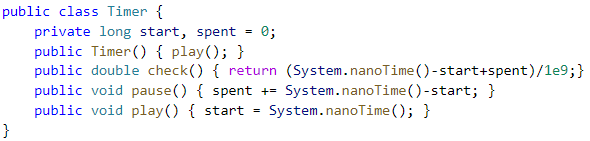
\includegraphics[]{figures/Figure-1.png}
    \label{fig:timer-class}
\end{figure}

\begin{figure}[h]
    \caption{Main.java}
    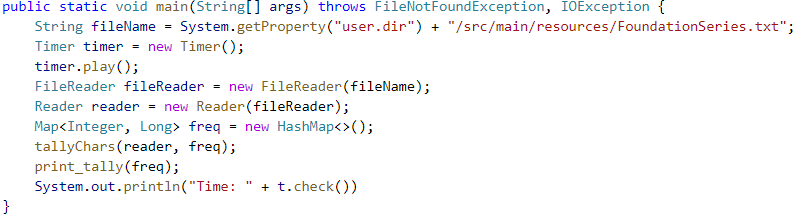
\includegraphics[]{figures/Figure-2.png}
    \label{fig:main-cass}
\end{figure}

With our timer implemented, we then ran the program for a total of 10 times and took the average of our timings to present a baseline of performance.\\\\

\begin{lstlisting}[]
Run 1:  152.073 ms
Run 2:  104.019 ms
Run 3:  66.9943 ms
Run 4:  88.3265 ms
Run 5:  64.8921 ms
Run 6:  52.9183 ms
Run 7:  53.6571 ms
Run 8:  53.3412 ms
Run 9:  96.7388 ms
Run 10: 87.2514 ms
\end{lstlisting}

\pagebreak
As we can see by our timings, the time to execute the program varies greatly.\\
The reason our timings are different for each run, is due to the pc running other processes during the test. In hindsight we should have run the test in a virtual environment to prevent any outside interferences, however by running the code 10 times and getting the average runtime we circumvent some of these interferences to get a clearer result.\\

We can now use our data to do a couple of different calculations to get an even even clearer picture of our programs performance before we improve upon it.\\
\begin{lstlisting}[]
Count:                  10
Sum:                    820.2117
Mean:                   82.02117
Variance:               866.8134585601
Standard Deviation:     29.441695918546
\end{lstlisting}
\pagebreak
\section{Bottlenecks and hypothesis of issues}


\subsection{Finding the bottlenecks}
To improve the programs performance, first of all we had to figure out what methods would give us the best performance increase once optimized.\\\\
We ran the program using intelliJ's built profiler named Flight Recorder to see which methods were the most performance heavy.

\begin{figure}[h]
    \caption{Profiler Flame Chart}
    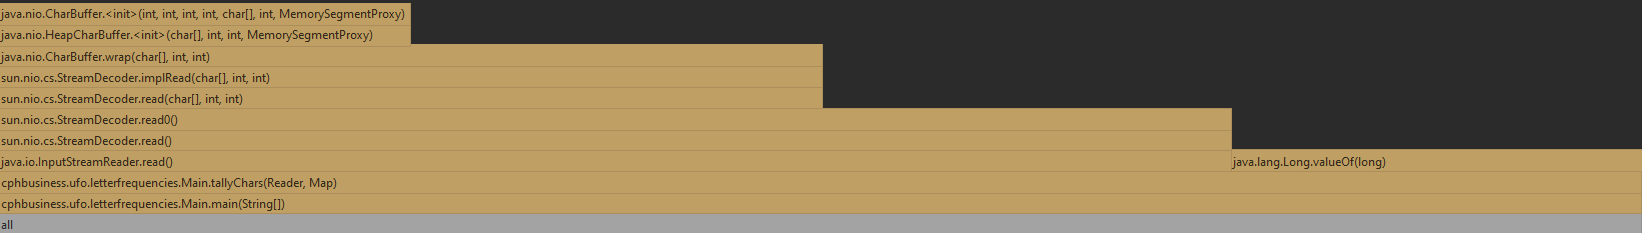
\includegraphics[width=\linewidth]{figures/java_profiler_unchanged_1.png}
    \label{fig:flame-chart-unchanged}
\end{figure}

\begin{figure}[h]
    \caption{Profiler Call Tree}
    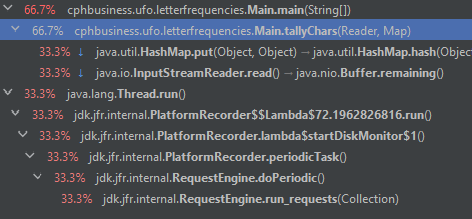
\includegraphics[width=\linewidth]{figures/java_profiler_unchanged_2.png}
    \label{fig:call-tree-unchanged}
\end{figure}

Looking at the charts, we clearly see that the "tallyChars" method  is the most costly function.\\\\
We ran the timer on the method 10 times and got an average of around 4.5ms, which is fairly high compared to other methods, therefor we decided to look further into it.

\newpage

\subsection{Hyphotesis - why is tallyChart so expensive}
The method is using a "Reader" to read data from a text file, which in our experience can be a costly method to run.
After an hour of extensively searching the internet, we came across a reputable source which explained that:

\begin{displayquote}
The new JDK 1.1 improves I/O performance with the addition of a collection of Reader and Writer classes. The readLine method in BufferedReader is at least 10 to 20 times faster than the one in DataInputStream when a large file is encountered. \parencite{how-to-improve-javas-io-performance}
\end{displayquote}

We replaced the old "Reader" with the new "BufferedReader" and gave it a max resource of 10.000 to satisfy it.  
\begin{figure}[h]
    \caption{Main.java with changed Reader type}
    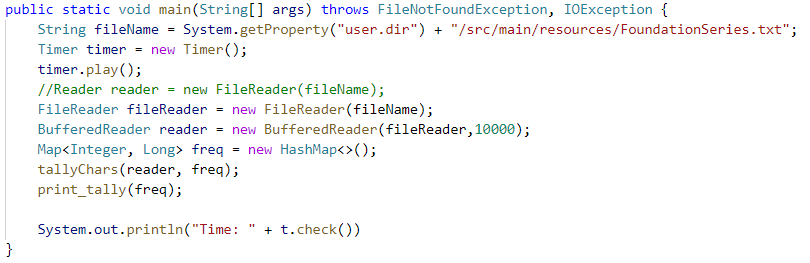
\includegraphics[width=\linewidth]{figures/Figure-3.png}
    \label{fig:flame-chart-unchanged}
\end{figure}

\begin{figure}[h]
    \caption{Main.java with updated tallyChars arguments}
    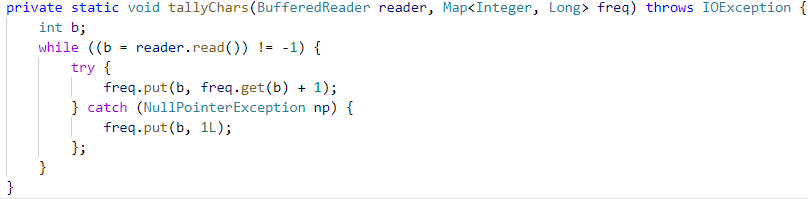
\includegraphics[width=\linewidth]{figures/Figure-4.png}
    \label{fig:flame-chart-unchanged}
\end{figure}

We performed the same test again with a marginal increase in performance.
\begin{lstlisting}[]
Run 1:  82.226 ms
Run 2:  34.3938 ms
Run 3:  58.0026 ms
Run 4:  40.7641 ms
Run 5:  30.4765 ms
Run 6:  39.6008 ms
Run 7:  41.5937 ms
Run 8:  42.4653 ms
Run 9:  52.4299 ms
Run 10: 39.8449 ms    
    \end{lstlisting}
\pagebreak
\section{Performance after optimization}
Lets check if our optimizations are indeed correct based on our research and current results.\\
We start out by once again, running the program program with a profiler.

\begin{figure}[h]
    \caption{Profiler Flame Chart}
    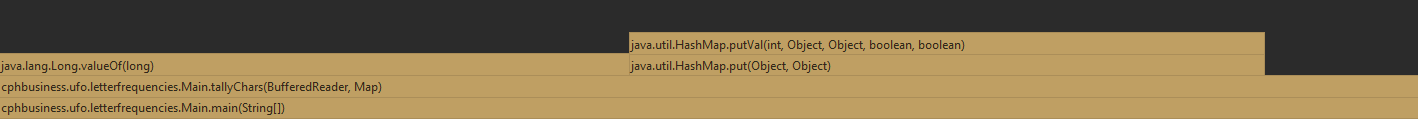
\includegraphics[width=\linewidth]{figures/java_profiler_changed_1.png}
    \label{fig:call-tree-unchanged}
\end{figure}

\begin{figure}[h]
    \caption{Profiler Flame Chart}
    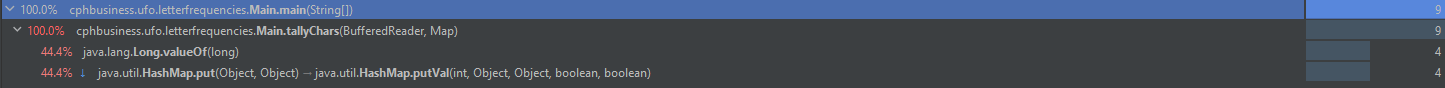
\includegraphics[width=\linewidth]{figures/java_profiler_changed_2.png}
    \label{fig:call-tree-unchanged}
\end{figure}

Just by looking at the profiler, it seems promising that our program will indeed be running less expensive.
To backup the profiler, we perform the same calculations as we did before the optimizations:

\begin{lstlisting}[]
        
        Optimized data

Count:                  10
Sum:                    461.7976
Mean:                   46.17976
Variance:               201.1248140124
Standard Deviation:     14.181848046443 
\end{lstlisting}

\vspace{30px}
Now lets compare it to our earlier results.
\vspace{20px}

\begin{lstlisting}[]        
        Unoptimized data

Count:                  10
Sum:                    820.2117
Mean:                   82.02117
Variance:               866.8134585601
Standard Deviation:     29.441695918546
\end{lstlisting}
\chapter{Conclusion}
As we can see from our data, small changes to the code can result in HUGE improvements to the execution times, which further reinforces our statement, that it is important to research the methods you're going to use before writing the program.\\\\

Our data confirms that we reached an average performance gain of 56.30\%, which is greater than our goal of reaching at least 50\% optimization.


\printbibliography

\end{document}